\documentclass[11pt]{article}

\usepackage[margin=1in]{geometry}
\usepackage{amsmath, amssymb, amsthm}
\usepackage{mathtools}
\usepackage{pgfplots}
\pgfplotsset{compat=1.17}
\usepackage{hyperref}
\hypersetup{colorlinks=true, linkcolor=blue!50!black, citecolor=blue!50!black}

\theoremstyle{definition}
\newtheorem{definition}{Definition}[section]
\newtheorem{example}[definition]{Example}
\newtheorem{remark}[definition]{Remark}
\theoremstyle{plain}
\newtheorem{proposition}[definition]{Proposition}

\newcommand{\Prob}{\mathbb{P}}
\newcommand{\E}{\mathbb{E}}
\newcommand{\dd}{\,\mathrm{d}}

\title{Survival and Hazard Functions}
\author{}
\date{}

\begin{document}
\maketitle

\begin{abstract}
These notes introduce the survival function and the hazard function of a nonnegative random variable, explain why the hazard function is a natural object for describing time-to-event data, and derive the relationships that allow each function to be recovered from the other. The continuous case is treated first; the discrete case is then used to give a second, more constructive derivation of the same result.
\end{abstract}

\tableofcontents

%======================================================================
\section{Setting and notation}
%======================================================================

Let $T$ be a nonnegative random variable representing the time until some event occurs. The event may be the death of a patient, the failure of a machine component, the default of a loan, or the cancellation of a subscription. Throughout Sections~\ref{sec:survival}--\ref{sec:examples} we assume that $T$ is absolutely continuous, with cumulative distribution function
\[
  F(t) = \Prob(T \le t), \qquad t \ge 0,
\]
and probability density function $f(t) = F'(t)$.

The distribution of $T$ is completely determined by either $F$ or $f$. The purpose of these notes is to introduce two further functions, the survival function and the hazard function, which also determine the distribution of $T$ but which are better suited to the questions that arise in the analysis of time-to-event data.

%======================================================================
\section{The survival function}\label{sec:survival}
%======================================================================

\begin{definition}[Survival function]
The \emph{survival function} of $T$ is
\[
  S(t) = \Prob(T > t) = 1 - F(t), \qquad t \ge 0.
\]
\end{definition}

The value $S(t)$ is the probability that the event has not yet occurred by time $t$. The following properties follow directly from the corresponding properties of $F$.

\begin{proposition}\label{prop:survival-props}
The survival function satisfies:
\begin{enumerate}
  \item $S(0) = 1$ (assuming $\Prob(T = 0) = 0$);
  \item $S$ is non-increasing;
  \item $S$ is right-continuous, and continuous when $T$ is absolutely continuous;
  \item $\lim_{t \to \infty} S(t) = 0$;
  \item $S'(t) = -f(t)$ wherever $f$ is continuous.
\end{enumerate}
\end{proposition}

The survival function also gives a convenient expression for the mean.

\begin{proposition}\label{prop:mean}
If $T \ge 0$, then
\[
  \E[T] = \int_0^\infty S(t) \dd t.
\]
\end{proposition}

\begin{proof}
Write $T = \int_0^\infty \mathbf{1}\{t < T\} \dd t$. Taking expectations and exchanging expectation and integral (justified by Tonelli's theorem, since the integrand is nonnegative) gives $\E[T] = \int_0^\infty \Prob(T > t) \dd t = \int_0^\infty S(t) \dd t$.
\end{proof}

Proposition~\ref{prop:mean} has a simple geometric reading: the mean survival time is the area under the survival curve.

%======================================================================
\section{Motivation for the hazard function}\label{sec:motivation}
%======================================================================

The density $f(t)$ answers the question: \emph{viewed from time zero}, how likely is the event to occur near time $t$? More precisely, for small $\Delta t > 0$,
\[
  \Prob(t \le T < t + \Delta t) \approx f(t)\,\Delta t.
\]

In many applications this is not the question of greatest interest. A physician treating a patient who has already survived five years after diagnosis does not want to know the unconditional probability of death in the sixth year; that probability is diluted by all the patients who did not survive to year five. The relevant quantity is the risk of the event in the near future \emph{given that it has not yet occurred}. Similarly, an engineer deciding whether to replace a component that has operated for 10{,}000 hours is concerned with the risk of failure for components of that age that are still working.

This suggests conditioning on survival to time $t$ and asking for the probability of the event in a short interval that follows:
\begin{equation}\label{eq:cond-prob}
  \Prob(t \le T < t + \Delta t \mid T \ge t).
\end{equation}
For small $\Delta t$ this probability is approximately proportional to $\Delta t$, so to obtain a quantity that does not depend on the arbitrary choice of interval length we divide by $\Delta t$ and take a limit. This leads to the following definition.

\begin{definition}[Hazard function]\label{def:hazard}
The \emph{hazard function} (also called the \emph{hazard rate}, \emph{failure rate}, or \emph{force of mortality}) of $T$ is
\begin{equation}\label{eq:hazard-def}
  h(t) = \lim_{\Delta t \downarrow 0}
  \frac{\Prob(t \le T < t + \Delta t \mid T \ge t)}{\Delta t},
  \qquad t \ge 0,
\end{equation}
wherever the limit exists.
\end{definition}

\begin{remark}\label{rem:not-probability}
The hazard $h(t)$ is a \emph{rate}, not a probability. It has units of $(\text{time})^{-1}$ and may exceed $1$. Its probabilistic interpretation is the approximation
\[
  \Prob(t \le T < t + \Delta t \mid T \ge t) \approx h(t)\,\Delta t
  \qquad \text{for small } \Delta t.
\]
Thus a hazard of $0.02$ per year means that, among individuals who have survived to time $t$, roughly $2\%$ will experience the event in the following year, provided the hazard does not change much over that year.
\end{remark}

%======================================================================
\section{From the survival function to the hazard function}\label{sec:s-to-h}
%======================================================================

We now express $h$ in terms of $f$ and $S$. By the definition of conditional probability,
\[
  \Prob(t \le T < t + \Delta t \mid T \ge t)
  = \frac{\Prob(t \le T < t + \Delta t)}{\Prob(T \ge t)}
  = \frac{F(t + \Delta t) - F(t)}{S(t)}.
\]
Here we have used $\Prob(T \ge t) = \Prob(T > t) = S(t)$, which holds because $\Prob(T = t) = 0$ for an absolutely continuous random variable. Substituting into~\eqref{eq:hazard-def},
\[
  h(t) = \frac{1}{S(t)} \lim_{\Delta t \downarrow 0}
  \frac{F(t + \Delta t) - F(t)}{\Delta t}
  = \frac{f(t)}{S(t)}.
\]

\begin{proposition}\label{prop:h-f-S}
For every $t$ with $S(t) > 0$ at which $f$ is continuous,
\begin{equation}\label{eq:h-f-S}
  h(t) = \frac{f(t)}{S(t)}.
\end{equation}
\end{proposition}

Equation~\eqref{eq:h-f-S} states precisely the intuition of Section~\ref{sec:motivation}: the hazard is the density rescaled by the fraction of the population still at risk. Where few individuals remain, even a small density corresponds to a large hazard.

Since $f(t) = -S'(t)$, equation~\eqref{eq:h-f-S} may be rewritten as
\begin{equation}\label{eq:h-log-S}
  h(t) = -\frac{S'(t)}{S(t)} = -\frac{\mathrm{d}}{\mathrm{d}t} \log S(t).
\end{equation}
This form shows that the hazard is the negative slope of the survival curve when the curve is plotted on a logarithmic scale.

%======================================================================
\section{From the hazard function to the survival function}\label{sec:h-to-s}
%======================================================================

Equation~\eqref{eq:h-log-S} is a first-order ordinary differential equation for $S$ with initial condition $S(0) = 1$. It can be solved directly.

\begin{definition}[Cumulative hazard]
The \emph{cumulative hazard function} is
\[
  H(t) = \int_0^t h(u) \dd u.
\]
\end{definition}

Integrating~\eqref{eq:h-log-S} from $0$ to $t$ gives
\[
  \int_0^t h(u) \dd u = -\bigl[\log S(u)\bigr]_0^t
  = -\log S(t) + \log S(0) = -\log S(t),
\]
since $\log S(0) = \log 1 = 0$. Exponentiating yields the central result.

\begin{proposition}\label{prop:S-exp-H}
For all $t \ge 0$,
\begin{equation}\label{eq:S-exp-H}
  S(t) = \exp\bigl(-H(t)\bigr) = \exp\!\left(-\int_0^t h(u) \dd u\right),
\end{equation}
and consequently
\begin{equation}\label{eq:f-h}
  f(t) = h(t)\,S(t) = h(t) \exp\!\left(-\int_0^t h(u) \dd u\right).
\end{equation}
\end{proposition}

The functions $F$, $f$, $S$, $h$, and $H$ therefore carry the same information: any one of them determines all the others. The relationships are summarized below.
\[
  \begin{array}{c|c}
    \text{Given} & \text{Recover} \\ \hline
    S & h = -(\log S)', \quad H = -\log S, \quad f = -S' \\[2pt]
    h & H = \int_0^t h, \quad S = e^{-H}, \quad f = h\,e^{-H} \\[2pt]
    f & S = \int_t^\infty f, \quad h = f/S
  \end{array}
\]

\begin{remark}[Which functions can be hazards?]\label{rem:valid-hazard}
Equation~\eqref{eq:S-exp-H} identifies the conditions a function must satisfy in order to be the hazard of some proper distribution on $[0,\infty)$. Since $S$ must lie in $[0,1]$ and be non-increasing, we need $h(t) \ge 0$. Since $S(t) \to 0$ as $t \to \infty$, we need
\[
  \int_0^\infty h(u) \dd u = \infty.
\]
Conversely, any nonnegative, locally integrable function with infinite total integral defines a valid distribution through~\eqref{eq:S-exp-H}. This is one practical advantage of modeling the hazard: the constraints are mild and easy to impose, whereas a density must integrate to exactly one. If $\int_0^\infty h < \infty$, then $S(\infty) = e^{-H(\infty)} > 0$, and the distribution is \emph{defective}: a positive fraction of the population never experiences the event. Such models are used deliberately in the study of diseases with a cured subpopulation.
\end{remark}

\subsection*{Conditional survival}

The exponential form also makes conditional survival probabilities easy to compute. For $s, t \ge 0$,
\begin{equation}\label{eq:cond-survival}
  \Prob(T > s + t \mid T > s)
  = \frac{S(s + t)}{S(s)}
  = \exp\!\left(-\int_s^{s+t} h(u) \dd u\right).
\end{equation}
The probability of surviving an additional $t$ units of time depends only on the hazard over the interval $(s, s+t]$. This is the formal counterpart of the statement that the hazard describes risk for those still at risk.

%======================================================================
\section{Examples}\label{sec:examples}
%======================================================================

\begin{example}[Exponential distribution]\label{ex:exponential}
Let $h(t) = \lambda$ for a constant $\lambda > 0$. Then $H(t) = \lambda t$,
\[
  S(t) = e^{-\lambda t}, \qquad f(t) = \lambda e^{-\lambda t},
\]
and $T$ is exponentially distributed with mean $1/\lambda$. By \eqref{eq:cond-survival},
\[
  \Prob(T > s + t \mid T > s) = e^{-\lambda t} = \Prob(T > t),
\]
which is the \emph{memoryless property}. A constant hazard means that an individual's age carries no information about its remaining lifetime. The exponential distribution is the only continuous distribution with this property, since~\eqref{eq:cond-survival} is independent of $s$ for all $t$ only when $h$ is constant.
\end{example}

\begin{example}[Weibull distribution]\label{ex:weibull}
Let $H(t) = (t/\lambda)^k$ with scale $\lambda > 0$ and shape $k > 0$. Then
\[
  S(t) = \exp\!\bigl(-(t/\lambda)^k\bigr), \qquad
  h(t) = \frac{k}{\lambda}\left(\frac{t}{\lambda}\right)^{k-1}.
\]
The shape parameter governs how risk changes with age:
\begin{itemize}
  \item $k < 1$: the hazard decreases. This describes \emph{infant mortality} or early failure, in which defective units fail quickly and the survivors are more robust.
  \item $k = 1$: the hazard is constant, and the Weibull reduces to the exponential distribution.
  \item $k > 1$: the hazard increases. This describes \emph{wear-out} or aging.
\end{itemize}
Figure~\ref{fig:weibull} displays the three cases.
\end{example}

\begin{figure}[ht]
\centering
\begin{minipage}{0.48\textwidth}
\centering
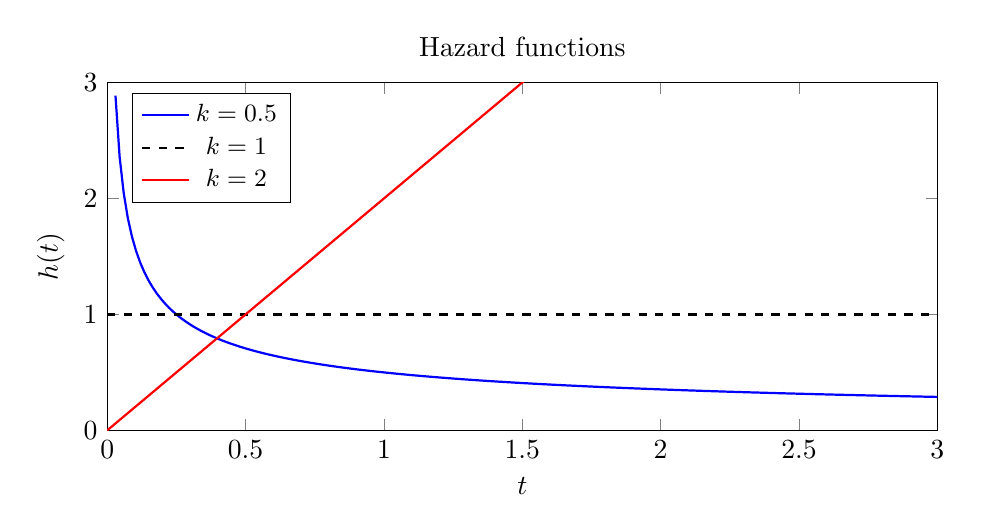
\begin{tikzpicture}
\begin{axis}[
  width=\linewidth, height=6cm,
  xlabel={$t$}, ylabel={$h(t)$},
  xmin=0, xmax=3, ymin=0, ymax=3,
  legend pos=north west, legend style={font=\small},
  title={Hazard functions}
]
\addplot[domain=0.03:3, samples=200, thick, blue]
  {0.5*x^(-0.5)};
\addlegendentry{$k=0.5$}
\addplot[domain=0:3, samples=2, thick, black, dashed]
  {1};
\addlegendentry{$k=1$}
\addplot[domain=0:3, samples=200, thick, red]
  {2*x};
\addlegendentry{$k=2$}
\end{axis}
\end{tikzpicture}
\end{minipage}\hfill
\begin{minipage}{0.48\textwidth}
\centering
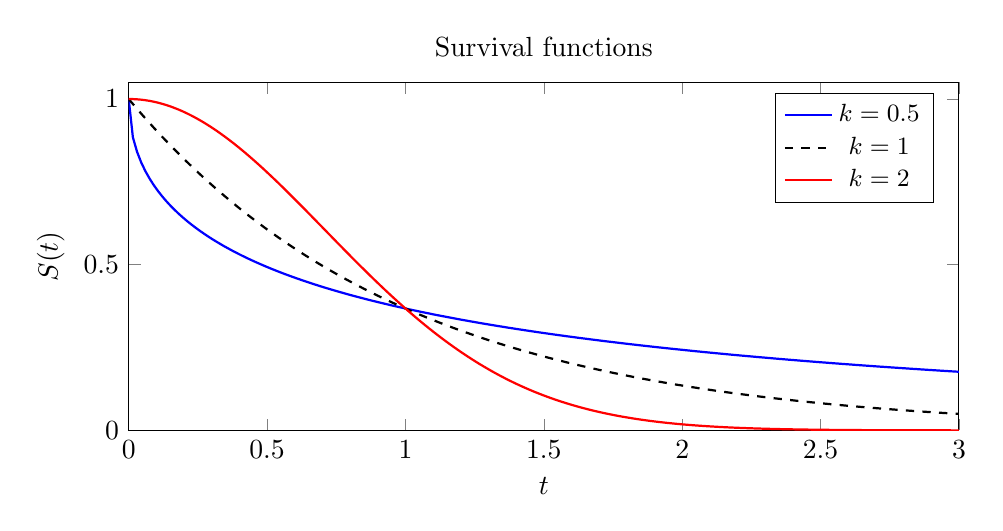
\begin{tikzpicture}
\begin{axis}[
  width=\linewidth, height=6cm,
  xlabel={$t$}, ylabel={$S(t)$},
  xmin=0, xmax=3, ymin=0, ymax=1.05,
  legend pos=north east, legend style={font=\small},
  title={Survival functions}
]
\addplot[domain=0:3, samples=200, thick, blue]
  {exp(-sqrt(x))};
\addlegendentry{$k=0.5$}
\addplot[domain=0:3, samples=200, thick, black, dashed]
  {exp(-x)};
\addlegendentry{$k=1$}
\addplot[domain=0:3, samples=200, thick, red]
  {exp(-x^2)};
\addlegendentry{$k=2$}
\end{axis}
\end{tikzpicture}
\end{minipage}
\caption{Weibull hazard and survival functions with $\lambda = 1$. All three survival curves pass through $S(1) = e^{-1}$, since $H(1) = 1$ for every $k$. Early on, the $k=0.5$ curve falls fastest because its hazard is largest; later the ordering reverses.}
\label{fig:weibull}
\end{figure}

\begin{example}[Bathtub hazards]
Many real systems, including human mortality over a full lifespan, exhibit a hazard that is high at first, falls to a low plateau, and then rises again. Such a \emph{bathtub-shaped} hazard can be constructed as a sum, for instance $h(t) = h_1(t) + h_2(t) + c$ with $h_1$ decreasing, $h_2$ increasing, and $c > 0$ constant. By~\eqref{eq:S-exp-H},
\[
  S(t) = e^{-H_1(t)}\,e^{-H_2(t)}\,e^{-ct},
\]
which is the survival function of $\min(T_1, T_2, T_3)$ for independent lifetimes $T_i$ with the respective hazards. Adding hazards thus corresponds to independent competing causes of failure, where the first cause to act determines the event time.
\end{example}

%======================================================================
\section{The discrete-time case}\label{sec:discrete}
%======================================================================

The continuous-time derivation, though short, relies on calculus identities that can obscure the underlying reasoning. The discrete case makes that reasoning explicit and shows where the exponential in~\eqref{eq:S-exp-H} comes from.

Suppose $T$ takes values in $\{t_1 < t_2 < \cdots\}$. Define the \emph{discrete hazard}
\[
  h_j = \Prob(T = t_j \mid T \ge t_j),
\]
which, unlike the continuous hazard, is a genuine probability. To survive past $t_j$, an individual must survive each of $t_1, \dots, t_j$ in turn. By the multiplication rule for conditional probabilities,
\begin{align*}
  S(t_j) = \Prob(T > t_j)
  &= \Prob(T > t_1)\,\Prob(T > t_2 \mid T > t_1) \cdots
     \Prob(T > t_j \mid T > t_{j-1}) \\
  &= \prod_{i=1}^{j} (1 - h_i).
\end{align*}
The survival function is therefore a product of conditional survival probabilities. This product form is the basis of the Kaplan--Meier estimator, in which each $h_i$ is estimated by the number of events at $t_i$ divided by the number of individuals at risk just before $t_i$.

\subsection*{Passage to the continuous limit}

Now let $T$ be continuous with hazard $h$, and partition $[0, t]$ into $n$ intervals of width $\Delta = t/n$ at points $u_i = i\Delta$. By Remark~\ref{rem:not-probability}, the conditional probability of the event in the $i$th interval, given survival to its start, is approximately $h(u_i)\Delta$. The discrete argument then gives
\[
  S(t) \approx \prod_{i=0}^{n-1} \bigl(1 - h(u_i)\,\Delta\bigr).
\]
Taking logarithms and using $\log(1 - x) = -x + O(x^2)$ as $x \to 0$,
\[
  \log S(t) \approx \sum_{i=0}^{n-1} \log\bigl(1 - h(u_i)\Delta\bigr)
  = -\sum_{i=0}^{n-1} h(u_i)\,\Delta + O\!\left(n \Delta^2\right).
\]
As $n \to \infty$, the sum is a Riemann sum converging to $\int_0^t h(u)\dd u$, and the error term $O(n\Delta^2) = O(t^2/n)$ vanishes. Hence
\[
  S(t) = \exp\!\left(-\int_0^t h(u) \dd u\right),
\]
in agreement with~\eqref{eq:S-exp-H}. The exponential is simply what a product of many factors of the form $1 - (\text{small})$ becomes in the limit. (In more advanced treatments, this limit is called a \emph{product integral}, and it provides a single formula for $S$ in terms of the cumulative hazard that is valid for continuous, discrete, and mixed distributions alike.)

%======================================================================
\section{Why the hazard is the natural modeling object}\label{sec:why}
%======================================================================

We close by noting two reasons, beyond interpretability, that time-to-event models are usually specified through the hazard.

\paragraph{Censoring.} In practice the event time is often not observed for every individual. A study may end, or a subject may be lost to follow-up, before the event occurs. For such a \emph{right-censored} individual we know only that $T > c$ for some censoring time $c$. Let $t_i$ denote the observed time for individual $i$ and let $\delta_i = 1$ if the event was observed and $\delta_i = 0$ if the observation was censored. Under the assumption that censoring is independent of the event process, individual $i$ contributes $f(t_i)$ to the likelihood if $\delta_i = 1$ and $S(t_i)$ if $\delta_i = 0$. Using~\eqref{eq:f-h}, the likelihood becomes
\[
  L = \prod_i f(t_i)^{\delta_i}\, S(t_i)^{1 - \delta_i}
    = \prod_i h(t_i)^{\delta_i} \exp\bigl(-H(t_i)\bigr).
\]
Every individual contributes the factor $e^{-H(t_i)}$, accounting for the time spent at risk, and only those with observed events contribute the additional factor $h(t_i)$. The hazard thus separates cleanly the information supplied by exposure time from the information supplied by events.

\paragraph{Covariates.} When the risk of the event depends on covariates $x$, it is often reasonable to suppose that covariates act multiplicatively on the hazard:
\[
  h(t \mid x) = h_0(t)\,\exp(\beta^\top x).
\]
This is the \emph{proportional hazards} model of Cox. The coefficient $\beta_j$ has the interpretation that a one-unit increase in $x_j$ multiplies the instantaneous risk by $e^{\beta_j}$ at every time $t$. Under this model, \eqref{eq:S-exp-H} gives $S(t \mid x) = S_0(t)^{\exp(\beta^\top x)}$, a relationship that would be difficult to state or motivate directly in terms of densities.

%======================================================================
\section{The counting-process formulation}\label{sec:counting}
%======================================================================

The treatment so far has regarded the event time $T$ as a single random variable whose distribution is to be described. This point of view becomes awkward as soon as the data are more complicated than a single, possibly censored, time per individual. Censoring times, covariates that change over time, repeated events, and delayed entry into a study all involve information that accumulates as time passes. The counting-process formulation, developed by Aalen in the 1970s, replaces the single random variable by a process that evolves in time and describes the risk of an event at each instant given everything observed up to that instant. The hazard function reappears in this setting as the rate of the process, and the estimators of Section~\ref{sec:discrete} and the likelihood of Section~\ref{sec:why} acquire a common structure.

The presentation below is heuristic. We work with infinitesimal increments $\mathrm{d}N(t)$ and conditional expectations given the past, and we omit the measure-theoretic conditions (predictability, the usual conditions on the filtration) required for a rigorous treatment. References are given at the end of the section.

\subsection{Counting processes and at-risk processes}

Consider $n$ individuals. For individual $i$ let $T_i$ be the event time and $C_i$ the censoring time, and suppose we observe
\[
  X_i = \min(T_i, C_i), \qquad \delta_i = \mathbf{1}\{T_i \le C_i\}.
\]
We encode these observations as two processes indexed by time.

\begin{definition}[Counting and at-risk processes]
The \emph{counting process} for individual $i$ is
\[
  N_i(t) = \mathbf{1}\{X_i \le t,\ \delta_i = 1\},
\]
which equals $0$ until an event is observed and jumps to $1$ at the time of the event. The \emph{at-risk process} is
\[
  Y_i(t) = \mathbf{1}\{X_i \ge t\},
\]
which equals $1$ while individual $i$ is under observation and could experience an observed event at time $t$. The aggregate processes are $N(t) = \sum_i N_i(t)$ and $Y(t) = \sum_i Y_i(t)$.
\end{definition}

Thus $N(t)$ counts the observed events up to time $t$, and $Y(t)$ is the size of the \emph{risk set} at time $t$. Note that $Y_i$ is defined with a non-strict inequality, so that $Y_i(t) = 1$ at the instant $t = X_i$. This makes $Y_i(t)$ known just before time $t$, which is the property needed below.

We write $\mathcal{F}_{t-}$ for the information available just before time $t$: which individuals have experienced events or been censored before $t$, and at what times, together with any covariate values observed so far. Formally, $(\mathcal{F}_t)_{t \ge 0}$ is a filtration, an increasing family of $\sigma$-algebras.

\subsection{The intensity process}

The key quantity is the conditional probability that individual $i$ has an observed event in $[t, t + \mathrm{d}t)$, given the past. If $Y_i(t) = 0$, the individual has already had the event or been censored, and this probability is zero. If $Y_i(t) = 1$, the individual is known to satisfy $T_i \ge t$ and $C_i \ge t$. We now make the central assumption.

\begin{definition}[Independent censoring]
Censoring is \emph{independent} if, for individuals still at risk, the conditional probability of an event in $[t, t + \mathrm{d}t)$ given $\mathcal{F}_{t-}$ equals $h(t)\,\mathrm{d}t$, the value it would have in the absence of censoring.
\end{definition}

Independent censoring states that the individuals who remain under observation are representative, as far as their immediate risk is concerned, of all individuals who have not yet experienced the event. It is implied by, but weaker than, stochastic independence of $T_i$ and $C_i$. Under this assumption, Remark~\ref{rem:not-probability} gives
\begin{equation}\label{eq:intensity}
  \E\bigl[\mathrm{d}N_i(t) \mid \mathcal{F}_{t-}\bigr]
  = \Prob\bigl(\mathrm{d}N_i(t) = 1 \mid \mathcal{F}_{t-}\bigr)
  = Y_i(t)\,h(t)\,\mathrm{d}t.
\end{equation}

\begin{definition}[Intensity and compensator]
The process $\lambda_i(t) = Y_i(t)\,h(t)$ is the \emph{intensity process} of $N_i$, and
\[
  \Lambda_i(t) = \int_0^t \lambda_i(u) \dd u = \int_0^t Y_i(u)\,h(u) \dd u
\]
is its \emph{compensator}.
\end{definition}

The intensity factors into a part describing the individual's observation status, $Y_i(t)$, and a part describing the underlying risk, $h(t)$. The compensator $\Lambda_i(t)$ is the cumulative hazard accumulated by individual $i$ over the period in which it was actually observed; compare the factor $e^{-H(t_i)}$ in the likelihood of Section~\ref{sec:why}.

\subsection{The martingale decomposition}

Define
\begin{equation}\label{eq:martingale}
  M_i(t) = N_i(t) - \Lambda_i(t).
\end{equation}
By~\eqref{eq:intensity},
\[
  \E\bigl[\mathrm{d}M_i(t) \mid \mathcal{F}_{t-}\bigr]
  = \E\bigl[\mathrm{d}N_i(t) \mid \mathcal{F}_{t-}\bigr] - \lambda_i(t)\dd t
  = 0.
\]
A process whose increments have conditional mean zero given the past is a \emph{martingale}. Summing increments over $(s, t]$ gives $\E[M_i(t) - M_i(s) \mid \mathcal{F}_s] = 0$, and in particular $\E[M_i(t)] = M_i(0) = 0$ for all $t$.

Equation~\eqref{eq:martingale} can be read as a decomposition of the observed data into signal and noise:
\[
  \underbrace{\mathrm{d}N_i(t)}_{\text{observed}}
  = \underbrace{\lambda_i(t)\dd t}_{\text{predictable given the past}}
  + \underbrace{\mathrm{d}M_i(t)}_{\text{unpredictable noise}}.
\]
This is the continuous-time analogue of writing a response in a regression model as its conditional mean plus an error with mean zero. The Doob--Meyer decomposition theorem guarantees that a decomposition of this form exists and is unique for any counting process; the hazard model specifies what the predictable part is.

The conditional variance of the noise is also determined by the intensity. Given $\mathcal{F}_{t-}$, the increment $\mathrm{d}N_i(t)$ is a Bernoulli variable with success probability $\lambda_i(t)\dd t$, so
\[
  \operatorname{Var}\bigl(\mathrm{d}M_i(t) \mid \mathcal{F}_{t-}\bigr)
  = \lambda_i(t)\dd t\,\bigl(1 - \lambda_i(t)\dd t\bigr)
  \approx \lambda_i(t)\dd t.
\]
Accumulating these conditional variances defines the \emph{predictable variation} $\langle M_i \rangle(t) = \Lambda_i(t)$. For $i \ne j$, the processes $N_i$ and $N_j$ do not jump simultaneously (for continuous event times), and $M_i$ and $M_j$ are \emph{orthogonal}: their increments are conditionally uncorrelated.

\subsection{Stochastic integrals}

Statistics used in survival analysis are typically weighted sums of the increments $\mathrm{d}N_i$. Let $K(t)$ be a process whose value at time $t$ is determined by $\mathcal{F}_{t-}$; such a process is called \emph{predictable}. Then
\[
  \E\bigl[K(t)\,\mathrm{d}M(t) \mid \mathcal{F}_{t-}\bigr]
  = K(t)\,\E\bigl[\mathrm{d}M(t) \mid \mathcal{F}_{t-}\bigr] = 0,
\]
because $K(t)$ is fixed once $\mathcal{F}_{t-}$ is known. It follows that the stochastic integral $\int_0^t K(u) \dd M(u)$ is again a martingale, with mean zero and predictable variation
\begin{equation}\label{eq:stoch-int-var}
  \left\langle \int K \dd M \right\rangle(t)
  = \int_0^t K(u)^2\,\lambda(u) \dd u.
\end{equation}
This single fact, that predictable weights preserve the martingale property, is the source of most of the unbiasedness and variance results that follow.

\subsection{The Nelson--Aalen estimator}

Summing~\eqref{eq:martingale} over individuals gives
\[
  \mathrm{d}N(t) = Y(t)\,h(t)\dd t + \mathrm{d}M(t),
  \qquad M = \sum_{i=1}^n M_i.
\]
Let $J(t) = \mathbf{1}\{Y(t) > 0\}$. Dividing by $Y(t)$ where it is positive suggests the estimator
\begin{equation}\label{eq:nelson-aalen}
  \widehat{H}(t) = \int_0^t \frac{J(u)}{Y(u)} \dd N(u)
  = \sum_{t_j \le t} \frac{d_j}{Y(t_j)},
\end{equation}
where $t_1 < t_2 < \cdots$ are the distinct observed event times and $d_j$ is the number of events at $t_j$. This is the \emph{Nelson--Aalen estimator} of the cumulative hazard. Each term $d_j / Y(t_j)$ is the natural estimate of the discrete hazard of Section~\ref{sec:discrete}: the fraction of those at risk who experienced the event.

To analyze $\widehat{H}$, define $H^*(t) = \int_0^t J(u)\,h(u) \dd u$, which equals $H(t)$ as long as someone remains at risk. Then
\[
  \widehat{H}(t) - H^*(t)
  = \int_0^t \frac{J(u)}{Y(u)} \bigl(\mathrm{d}N(u) - Y(u)\,h(u)\dd u\bigr)
  = \int_0^t \frac{J(u)}{Y(u)} \dd M(u).
\]
The weight $J(u)/Y(u)$ is predictable, since the size of the risk set at time $u$ is known just before $u$. The estimation error is therefore a stochastic integral with respect to a martingale, and we obtain the following.

\begin{proposition}\label{prop:nelson-aalen}
Under independent censoring,
\begin{enumerate}
  \item $\E\bigl[\widehat{H}(t) - H^*(t)\bigr] = 0$, so $\widehat{H}(t)$ is unbiased for $H^*(t)$;
  \item by~\eqref{eq:stoch-int-var}, the predictable variation of the error is
        \[
          \int_0^t \frac{J(u)^2}{Y(u)^2}\,Y(u)\,h(u) \dd u
          = \int_0^t \frac{J(u)\,h(u)}{Y(u)} \dd u,
        \]
        which is estimated by replacing $h(u)\dd u$ with $\mathrm{d}\widehat{H}(u)$:
        \[
          \widehat{\sigma}^2(t) = \int_0^t \frac{J(u)}{Y(u)^2} \dd N(u)
          = \sum_{t_j \le t} \frac{d_j}{Y(t_j)^2}.
        \]
\end{enumerate}
\end{proposition}

The variance formula has a direct interpretation: an event observed when few individuals are at risk contributes a large term, reflecting the fact that hazard estimates late in follow-up rest on little data. Large-sample normality of $\sqrt{n}\,\bigl(\widehat{H}(t) - H(t)\bigr)$ follows from a central limit theorem for martingales due to Rebolledo, which requires only that the predictable variation converge to a deterministic limit and that individual jumps become negligible.

\begin{remark}[Relation to Kaplan--Meier]
Section~\ref{sec:discrete} showed that the survival function is the product of conditional survival probabilities. Applying that product to the increments of the Nelson--Aalen estimator gives
\[
  \widehat{S}(t) = \prod_{t_j \le t} \bigl(1 - \Delta\widehat{H}(t_j)\bigr)
  = \prod_{t_j \le t} \left(1 - \frac{d_j}{Y(t_j)}\right),
\]
which is the Kaplan--Meier estimator. The two classical nonparametric estimators are thus related exactly as $S$ and $H$ are related through the product integral. The alternative $\exp\bigl(-\widehat{H}(t)\bigr)$, which mimics~\eqref{eq:S-exp-H} directly, is also used and is close to $\widehat{S}(t)$ when the increments $d_j / Y(t_j)$ are small.
\end{remark}

\subsection{The Cox partial likelihood}

Suppose now that individual $i$ has a covariate vector $x_i(t)$, which may vary with time provided its value at $t$ is known just before $t$. The proportional hazards model of Section~\ref{sec:why} specifies the intensity
\[
  \lambda_i(t) = Y_i(t)\,h_0(t)\,\exp\bigl(\beta^\top x_i(t)\bigr),
\]
where the baseline hazard $h_0$ is left unspecified. Define
\[
  S^{(0)}(\beta, t) = \sum_{j=1}^n Y_j(t)\,e^{\beta^\top x_j(t)}, \qquad
  S^{(1)}(\beta, t) = \sum_{j=1}^n Y_j(t)\,x_j(t)\,e^{\beta^\top x_j(t)}, \qquad
  S^{(2)}(\beta, t) = \sum_{j=1}^n Y_j(t)\,x_j(t)\,x_j(t)^{\!\top}\,e^{\beta^\top x_j(t)},
\]
and $\bar{x}(\beta, t) = S^{(1)}(\beta, t) / S^{(0)}(\beta, t)$, which is a weighted average of the covariates over the risk set.

Given that exactly one event occurs at time $t$, the conditional probability that it is individual $i$ is the ratio of intensities,
\[
  \frac{\lambda_i(t)}{\sum_j \lambda_j(t)}
  = \frac{Y_i(t)\,e^{\beta^\top x_i(t)}}{S^{(0)}(\beta, t)}.
\]
The unknown baseline $h_0(t)$ cancels. Multiplying these probabilities over the observed event times gives the \emph{partial likelihood}
\[
  L(\beta) = \prod_{i=1}^n \prod_{t \ge 0}
  \left(\frac{Y_i(t)\,e^{\beta^\top x_i(t)}}{S^{(0)}(\beta, t)}\right)^{\mathrm{d}N_i(t)},
\]
where the inner product has at most one factor different from $1$. Its logarithm and score function are
\[
  \log L(\beta) = \sum_{i=1}^n \int_0^\infty
    \Bigl(\beta^\top x_i(u) - \log S^{(0)}(\beta, u)\Bigr) \dd N_i(u),
\]
\[
  U(\beta) = \sum_{i=1}^n \int_0^\infty
    \bigl(x_i(u) - \bar{x}(\beta, u)\bigr) \dd N_i(u).
\]
The score compares, at each event time, the covariate of the individual who failed with the average covariate among those at risk.

The counting-process formulation now explains why the score has mean zero at the true parameter $\beta_0$, which is the property on which consistency of the maximum partial likelihood estimator rests. Substitute $\mathrm{d}N_i(u) = \lambda_i(u)\dd u + \mathrm{d}M_i(u)$. The compensator term is
\[
  \sum_{i=1}^n \bigl(x_i(u) - \bar{x}(\beta_0, u)\bigr)\,
    Y_i(u)\,h_0(u)\,e^{\beta_0^\top x_i(u)}
  = h_0(u)\Bigl(S^{(1)}(\beta_0, u) - \bar{x}(\beta_0, u)\,S^{(0)}(\beta_0, u)\Bigr)
  = 0,
\]
by the definition of $\bar{x}$. Therefore
\[
  U(\beta_0) = \sum_{i=1}^n \int_0^\infty
    \bigl(x_i(u) - \bar{x}(\beta_0, u)\bigr) \dd M_i(u),
\]
a sum of stochastic integrals of predictable processes with respect to orthogonal martingales. It has mean zero, and by~\eqref{eq:stoch-int-var} its predictable variation is
\[
  \sum_{i=1}^n \int_0^\infty
    \bigl(x_i - \bar{x}\bigr)\bigl(x_i - \bar{x}\bigr)^{\!\top} \lambda_i(u) \dd u
  = \int_0^\infty
    \left(\frac{S^{(2)}(\beta_0, u)}{S^{(0)}(\beta_0, u)}
      - \bar{x}(\beta_0, u)\,\bar{x}(\beta_0, u)^{\!\top}\right)
    S^{(0)}(\beta_0, u)\,h_0(u) \dd u.
\]
Replacing $S^{(0)}(\beta_0, u)\,h_0(u)\dd u$, the compensator of the aggregate counting process, with $\mathrm{d}N(u)$ gives
\[
  \int_0^\infty
    \left(\frac{S^{(2)}(\beta, u)}{S^{(0)}(\beta, u)}
      - \bar{x}(\beta, u)\,\bar{x}(\beta, u)^{\!\top}\right) \dd N(u),
\]
which is exactly the observed information $-\partial U / \partial \beta$. The partial likelihood therefore has the same score-and-information structure as an ordinary likelihood, even though it is not the full likelihood of the data, and the usual Wald, score, and likelihood-ratio procedures are justified by the martingale central limit theorem.

\subsection{Scope of the formulation}

The results above used only three ingredients: the counting processes $N_i$, the at-risk indicators $Y_i$, and a model for the intensity $\lambda_i$. Several extensions of the basic survival setting amount to changing the definition of $Y_i$ or $\lambda_i$ while leaving the theory intact.
\begin{itemize}
  \item \emph{Delayed entry.} If individual $i$ enters observation at time $L_i > 0$, set $Y_i(t) = \mathbf{1}\{L_i < t \le X_i\}$.
  \item \emph{Recurrent events.} If individual $i$ can experience the event repeatedly, let $N_i(t)$ count all events up to $t$ and let $Y_i(t)$ remain $1$ after each event until censoring.
  \item \emph{Time-varying covariates.} These enter the intensity directly, as in the Cox model above, provided they are predictable.
  \item \emph{Competing risks and multistate models.} Each type of transition receives its own counting process and intensity, with the at-risk indicator recording whether the individual currently occupies the state from which that transition is possible.
\end{itemize}
In each case the estimators have the form of~\eqref{eq:nelson-aalen} or of the partial likelihood score, and their properties follow from the martingale decomposition in the same way.

\paragraph{Further reading.} The standard references are Andersen, Borgan, Gill, and Keiding, \emph{Statistical Models Based on Counting Processes} (Springer, 1993), and Fleming and Harrington, \emph{Counting Processes and Survival Analysis} (Wiley, 1991), both of which give rigorous treatments. Aalen, Borgan, and Gjessing, \emph{Survival and Event History Analysis: A Process Point of View} (Springer, 2008), is more accessible and emphasizes interpretation.

%======================================================================
\section*{Exercises}
%======================================================================

\begin{enumerate}
  \item Show that if $h(t) = \alpha e^{\gamma t}$ with $\alpha, \gamma > 0$ (the Gompertz hazard), then $S(t) = \exp\bigl(-\tfrac{\alpha}{\gamma}(e^{\gamma t} - 1)\bigr)$. Why has this model been widely used for adult human mortality?
  \item Let $T_1$ and $T_2$ be independent with hazards $h_1$ and $h_2$. Show that $\min(T_1, T_2)$ has hazard $h_1 + h_2$.
  \item Compute the hazard of the log-logistic distribution, $S(t) = 1/(1 + (t/\alpha)^\beta)$, and show that for $\beta > 1$ it first increases and then decreases. Give an application in which such a shape would be plausible.
  \item The \emph{mean residual life} is $m(t) = \E[T - t \mid T > t]$. Show that $m(t) = \int_t^\infty S(u)\dd u \,/\, S(t)$, and verify that $m(t)$ is constant for the exponential distribution.
  \item Suppose $h(t) = 1/(1 + t)$. Compute $\int_0^\infty h(t)\dd t$ and determine whether this defines a proper distribution. What is $\E[T]$?
\end{enumerate}

\end{document}
